\documentclass{article}
\usepackage{tikz}
\begin{document}
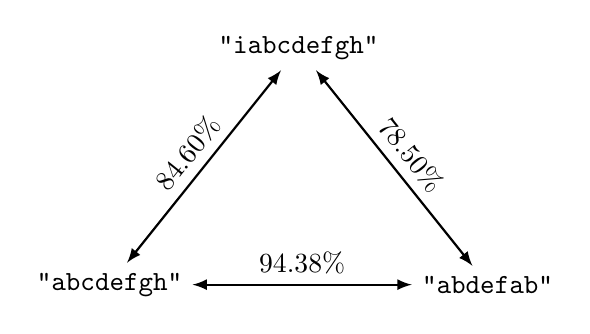
\begin{tikzpicture}[>=latex,thick]
    \node (a) at (0,0) {\texttt{"abcdefgh"}};
    \node (b) at (4.8,0) {\texttt{"abdefab"}};
    \node (c) at (2.4,3) {\texttt{"iabcdefgh"}};
    \draw[<->] (a)--node[above,sloped] {94.38\%} (b);
    \draw[<->] (a)--node[above,sloped] {84.60\%}(c);
    \draw[<->] (c)--node[above,sloped] {78.50\%}(b);
\end{tikzpicture}
\end{document}
